\section{Appendix}

\subsection{Selected basics of category theory}

\begin{definition}[\textbf{set}] 
\label{def:set}
A \textbf{set} $S$ is a collection of elements, with no specific operation or ordering.
\end{definition}

\begin{definition}[\textbf{structured set}] 
\label{def:structure}
A structured set (also called an object) is a set equipped with specific operations of elements in the set.
\end{definition}


\begin{example}
%
Two examples of commonly seen structured sets:
%
\begin{itemize}
    \item A \textbf{group} $G$ is a set, equipped with a binary operation, denoted as $(\cdot)$ or none, satisfying three axioms: the identity element, the inverse element and associativity $(\g_1\g_2)\g_3 = \g_1(\g_2\g_3)$.
    \item A \hyperref[def:vector-space]{\textbf{\underline{vector space}}} $\VF$ is a set, equipped with two operations:
    %
    \begin{itemize}
        \item addition in $\mathcal{V}$ (denoted as $+$, satisfying four axioms: the additive identity, additive inverse, additive commutativity  and additive associativity); \textcolor{red}{(So far, over this operation addition, $\mathcal{V}$ an be treated as an abelian group; note that $\F$ is not yet involved)} 
        \item scalar multiplication over field $\F$ (denoted as $\cdot$, satisfying four axioms: the scalar multiplicative identity, vector distributability, field additive distributability, field multiplicative compatibility). \textcolor{red}{(such extra properties makes $\VF$ more than a group, thereby distinct significantly from the characteristics of groups.)}
    \end{itemize}
    %
\end{itemize}
%
\end{example}


\begin{definition}[\textbf{homomorphism}] 
\label{def:homomorphism}
\label{def:map}
A homomorphism from a structured set  $X$ to a structured set $Y$ is a 
\annotate[id=b,comment={ A \textbf{map} (or called a \textbf{function}) from a set $X$ to a set $Y$ assigns each element of $X$ to exactly one element of $Y$.
Here, the set $X$ is called a domain, the set $Y$ is called a codomain.}]{map} that \textbf{preserves} the structure of $X$ and $Y$.
If there exists such a map between $X$ and $Y$, we say $X$ is homomorphic to $Y$, denoted as $X \backsim Y$.\\
\end{definition}
%
\begin{remark}
When $X$ and $Y$ are groups, the homomorphism is called a \textbf{group homomorphism}. 
When $X$ and $Y$ are vector spaces, the homomorphism is called a \textbf{linear map}.  
\end{remark}
%
\begin{figure}[h]
    \centering
    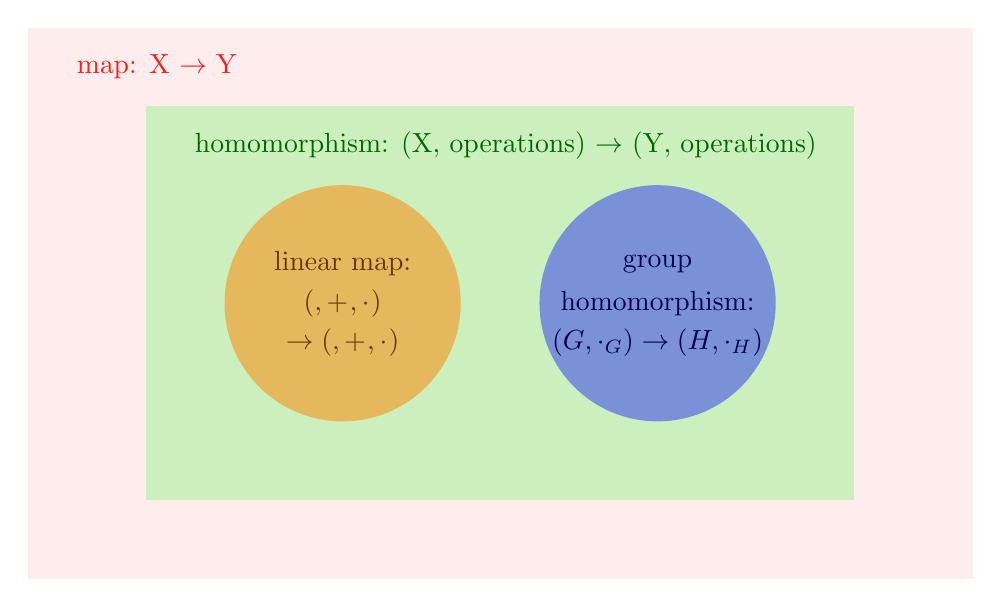
\begin{tikzpicture}
    %
    \begin{scope}
    % circles and a rectangle
        \fill[red!70!, opacity=0.1] (-6,-3.5) rectangle (6,3.5); % map
        \fill[green!100!black, opacity=0.2] (-4.5,-2.5) rectangle (4.5,2.5); % map
        \fill[orange!100!black, opacity=0.5] (0:-2) circle (1.5); % linear map
        \fill[blue!100!black, opacity=0.4] (0:2) circle (1.5); % group homomorphism
    \end{scope}
    %
    \node (map)[text=red!90!, anchor=west] at (-5.5, 3) {map: X $\to$ Y};
    \node (homomorphism)[text=green!40!black, anchor=west] at (-4, 2) {homomorphism: (X, operations) $\to$ (Y, operations) };
    \node (linear map)[text=orange!40!black] at (-2, 0.5) {linear map:};
    \node [text=orange!40!black] at (-2, -0) {$(\VF, +_{\VF}, \cdot_{\VF})$ };
    \node [text=orange!40!black] at (-2, -0.5) {$\to (\WF, +_{\WF}, \cdot_{\WF})$ };
    \node (group homomorphism)[text=blue!30!black] at (2, 0.5) {group};
    \node [text=blue!30!black] at (2, 0) {homomorphism:};
    \node [text=blue!30!black] at (2, -0.5) {$(G, \cdot_{G}) \to (H, \cdot_{H})$ };
    %
    \end{tikzpicture}
    \caption{Vienn diagram of maps}
    \label{fig:map-hormorphism}
\end{figure}



\begin{remark}[group homomorphism]
To check that a map $\f: (G, \cdot_G) \to (H, \cdot_H)$ ($G$ and $H$ are groups) is a group homomorphism, only need to verify that the binary operation is preserved under the map $\f$, i.e., the following operation
$$\f(g_1 \cdot_G g_2) = \f(g_1) \cdot_H \f(g_2).$$
Once so, it follows immediately that all \textbf{three} axioms of groups are preserved under the map:
\begin{enumerate}
    \item correspondence between the identity in $G$ and in $H$: $\f(g) = \f(e_{G} \cdot_G g) = \f(e_{G}) \cdot_H \f(g) \implies \f(e_{G}) = e_{H}$;
    \item correspondence between the inverse in $G$ and in $H$: $e_{H} = \f(e_{G}) = \f(g \cdot_G g^{-1})= \f(g) \cdot_H \f(g^{-1}) \implies  \forall g \in G, \f(g^{-1}) = \f(g)^{-1}$; 
    \item preservation of the associativity: $(g_1 \cdot_G g_2) \cdot_G g_3 = g_1 \cdot_G (g_2 \cdot_G g_3)  \Longleftrightarrow [\f(g_1) \cdot_H  \f(g_2)] \cdot_H \f(g_3) =  \f(g_1) \cdot_H [\f(g_2) \cdot_H \f(g_3)]$.
\end{enumerate}
%
\end{remark}
%
\begin{remark}[linear map]
To check if a map $\f: (\VF, +_{\VF}, \cdot_{\VF}) \to (\WF, +_{\WF}, \cdot_{\WF})$ ($\VF$ and $\WF$ are vector spaces) is linear, need to verify that the map preserves addition and scalar multiplication, i.e., the operations below
$$\f( \x +_{\VF} \y ) = \f(\x) +_{\WF} \f(\y),$$
$$\f(c \cdot_{\VF} \x) = c \cdot_{\VF} \f(\x),$$
for $\forall \x, \y \in \VF$ and $\forall c \in \F$. \\
Once so, it follows immediately that all \textbf{eight} axioms of vector spaces are preserved under the map:
\begin{enumerate}
    \item correspondence between the additive identity in $\VF$ and in $\WF$: $\f(\x) = \f(\x +_{\VF} \e_{\V}) = \f(\x) +_{\WF} \f(\e_{\V}) \implies \f(\e_{\V}) = \e_\W$;
    \item correspondence between the additive inverse in $\VF$ and in $\WF$: $\f(\e_{\V}) = \f[\x +_{\VF} (-\x)] = \f(\x) +_{\WF} \f(-\x) \implies \forall \x \in \VF, \f(-\x) = - \f(\x)$;
    \item commutativity of vector addition:  $\x_1 +_{\VF} \x_2 = \x_2 +_{\VF} \x_1 \Longrightarrow \f(\x_1) +_{\WF} \f(\x_2) = \f(\x_2) +_{\WF} \f(\x_1)$;
    \item associativity of vector addition: $ (\x_1 +_{\VF} \x_2) +_{\VF} \x_3 =  \x_1 +_{\VF} (\x_2 +_{\VF} \x_3) \Longrightarrow [\f(\x_1) +_{\WF} \f(\x_2)] +_{\WF} \f(\x_3) = \f(\x_1) +_{\WF} [\f(\x_2) +_{\WF} \f(\x_3)]$;
    \item correspondence between the scalar multiplicative identity in $\VF$ and in $\WF$: $\forall \x \in \VF, \f(\x) = \f(e_\V \cdot_{\VF}  \x) = e_\V \cdot_{\WF} \f(\x) \implies e_\V = e_\W \in \F$;
    \item compatibility of scalar multiplication with field multiplication: $\forall c_1,c_2 \in \F, \f[c_1 (c_2\x)] = c_1 \f(c_2\x) = (c_1 c_2) \f(\x)$;
    \item distributivity of scalar multiplication with respect to vector addition: $\forall \x,\y \in \VF, \f[c (\x + \y)] = \f(c\x + c\y) = \f(c\x) + \f(c\y) = c\f(\x) + c\f(\y)$;
    \item distributivity of scalar multiplication with respect to field addition: $\forall c_1,c_2 \in \F, \f[(c_1+c_2) \x] = \f(c_1\x + c_2\x) = \f(c_1\x) + \f(c_2\x) = c_1\f(\x) + c_2\f(\x)$;

\end{enumerate}
%
\end{remark}
%
\begin{remark}
A homomorphism implies:
\begin{align*}
    &\bullet \textnormal{that the structure of the domain is preserved in the image;}\\
    &\bullet \textnormal{nothing between the cardinalities of the domain and codomain}.
\end{align*}
\end{remark}
%

\begin{definition}[\textbf{isomorphism}] 
\label{def:isomorphism}
An isomorphism is a 
\annotate[id=b, comment = {bijective = injective + surjective.\\
A map $\f: X \to Y$ is injective, iff $\operatorname{ker}(\f) = \{e\}$; surjective, iff $\operatorname{imag}(\f) = Y$.}]{\textbf{bijective}} \hyperref[def:homomorphism]{homomorphism}, denoted as $X \cong Y$.
\end{definition}
%
\begin{remark}
An isomorphism implies:
\begin{align*}
    &\bullet \textnormal{structure preserved;}\\
    &\bullet \textnormal{same cardinality of the two sets}.
\end{align*}
An isomorphism between vector spaces $\VF$ and $\WF$ is a bijective linear map.\\
An isomorphism between two groups $G_1$ and $G_2$ is a bijective group homomorphism.
\end{remark}

\begin{theorem}[\textbf{quotient homomorphism}]
A homomorphism (either a group homomorphism or a linear map) $\f: X \to Y$ must satisfy 
$$\frac{X}{\operatorname{ker}(\f)} \cong \operatorname{imag}(\f),$$
where the left-hand side is called a \textbf{quotient group} (or a \textbf{quotient space}).
\end{theorem}
%
\begin{corollary}
If a  homomorphism $\f$ is injective, then $\operatorname{ker}(\f) = \{e\}$, thereby
$$X \cong \operatorname{imag}(\f).$$
If $\f$ is surjective, then $\operatorname{imag}(\f) = Y$ thereby
$$\frac{X}{\operatorname{ker}(\f)} \cong Y.$$
\end{corollary}



\subsection{Basics of linear maps}

\begin{definition}[\textbf{vector space}] 
\label{def:vector-space}
Given some field $\mathcal{F}$, a set $\mathcal{V}$ is called a \textbf{\underline{vector space}} over the field $\mathcal{F}$ if the operations of addition and scalar multiplication are defined on $\mathcal{V}$ such that 
$$ \x + \y \in \mathcal{V} \>\> \text{and} \,\,\, c\x \in \mathcal{V}$$
for any $ \x, \y \in \mathcal{V}$ and $c \in \mathcal{F}$. 
\end{definition}

\begin{remark}
\textbf{Without a field}, vector space cannot be defined.
To emphasise the significance of the field, in this note I call the vector space $\mathcal{V}$ over the field $\mathcal{F}$ by $\VF$.
\end{remark}

\begin{definition}[\textbf{basis of a vector space}]
A collection of vectors $\{v_i\}_i$ in the vector space $\VF$ constitute a \textbf{basis} of $\VF$ if $\{v_i\}_i$ contains the \textbf{least} number of elements that can \textbf{span} the vector space $\VF$, i.e., 
\begin{enumerate}
    \item \textbf{uniqueness}: any nonzero vector in $\VF$ is uniquely determined by a linear combination\footnote{result of vectors that are added and/or scalarly multiplied.} of $\{v_i\}_i$;
    \item \textbf{least number}: any other collection of vectors $\{w_i\}_i$ that satisfies the previous condition has no less elements than $\{v_i\}_i$.
\end{enumerate}
\end{definition}

\begin{definition}[\textbf{dimensionality of a vector space}]
The \textbf{dimension} of a vector space $\VF$ is the dimension of the basis of $\VF$, i.e., the number of elements in a basis of $\VF$.
\end{definition}


\begin{definition}[\textbf{map}]
The \textbf{dimension} of a vector space $\VF$ is the dimension of the basis of $\VF$, i.e., the number of elements in a basis of $\VF$.
\end{definition}


\note[id=b]{
Example:\\
the dimension of vector space $\mathbb{R}^2$ over field $\mathbb{R}$ is 2; \\
the dimension of vector space $\mathbb{C}$ over field $\mathbb{R}$ is 2; \\
the dimension of vector space $\mathbb{C}$ over field $\mathbb{C}$ is 1.\\
Examine the dimensionality by looking for a basis.}


\begin{textremark*}{Motivating Linearity}
A map links \textbf{elements} --- projecting any element in domain (some set $A$) to some element in codomain (some set $B$), while a \underline{\textbf{linear}} map also links \textbf{relationships between elements} --- projecting the additive ($+$) and scalar multiplicative ($\cdot$) operations within domain to those within codomain.\\
Motivated by such difference, we note that \\
$\bullet$ firstly, the domain and codomain of a linear map have to be (at least) vector spaces, not just sets, because otherwise $+$ and $\cdot$ are not equipped.\\
$\bullet$ secondly, for domain $(\VF, +_{\VF}, \cdot_{\VF})$ and codomain $(\WF, +_{\WF}, \cdot_{\WF})$ of a map $\f$:\\
$\f: \x +_{\VF} \y \mapsto \f(\x) +_{\WF} \f(\y)$ is not trivial;\\
$\f: c \cdot_{\VF} \x \mapsto c \cdot_{\WF} \f(\x)$ is not trivial.\\
It needs to be specifically defined.
\end{textremark*}

\begin{definition}[\textbf{linear map}] 
\label{def:linear-map}
A \hyperref[def:map]{map} from $\f(\cdot)$ from the vector space $\VF$ to the vector space $\WF$ is \textbf{linear} if addition and scalar multiplication are preserved under this map, i.e., 
$$\f( \x + \y ) = \f(\x) + \f(\y),$$
$$\f(c \x) = c \f(\x),$$
for $\x, \y \in \VF$ and $c \in \mathcal{F}$. 
\end{definition}
%
\begin{remark}\label{remark:linearmap}
%
\noindent 
%
\begin{itemize}
    \item The codomain must \textbf{share the same field} $\F$ as that of the domain, because in $$\f(c \x) = c \f(\x),$$
    we have $c \in \F_1$ the field of the domain and $c \in \F_2$ the field of the codomain.
    \item The structure-preserving property suggests the correspondence of the domain basis to the codomain. 
    Therefore, the dimension of $imag(f)$ must be the same as the domain $\VF$, i.e., there exists a bijection between the effective codomain $imag(f)$ and the domain $\VF$:
    $$imag(f) \cong \VF.$$
    It does no harm to the map if we replace the codomain $\WF$ by $imag(f)$.
    Therefore, \textbf{the codomain is usually the same as the domain, or isomorphic to it}.
    \item Example: fixing a shared field $\R$, a linear map $f: \R^2 \to \R^3$ is a homomorphism from a vector space $\R^2$ to another vector space $\R^3$.
    Since $imag(f) \subset \R^3$ is a vector space of dimension $2$, we know that $imag(f) \cong \R^2 \cong \mathbb{C}$.
    It does no harm to the structure-preserving property of the linear map, if we replace the codomain by $\R^2$ or $\mathbb{C}$.
\end{itemize}
%
\end{remark}

\begin{example}
Question: is $\mathbb{R}^2$ \hyperref[def:isomorphism]{isomorphic} to $\mathbb{C}$?\\
Answer: It depends.
Firstly, $\mathbb{R}^2 \cong \mathbb{C}$ means there exists a bijective linear map between them.
Secondly, for a map to be ``linear'', a shared field of domain and codomain is a must, so $\mathbb{R}^2$ over field $\mathbb{R}$ and $\mathbb{C}$ over field $\mathbb{C}$ are NOT isomorphic.
Finally, $\mathbb{R}^2$ over $\mathbb{R}$ and $\mathbb{C}$ over $\mathbb{R}$ are isomorphic.\\
In most cases, the field of vector spaces $\mathbb{R}^n$ and $\mathbb{C}$ are assumed by default to be $\R$.
\end{example}

\begin{proposition}[\textbf{matrix of a linear map}] \label{matrix of a linear map}
Any linear map has a unique matrix representation under a chosen basis of the domain and a chosen basis of codomain.
\end{proposition}

\begin{proof} 
For a linear map $\f(\cdot): \VF \to \WF$  (assuming finite dimensions of domain and codomain), choose a basis $\mathcal{A} = \{\b{a}_i\}_{i=1}^N$ of $\VF$ and a basis $\mathcal{B} = \{\b{b}_i\}_{i=1}^M$ of $\WF$. 

Let $\y_j := \f(\b{a}_j)$ for $i \in \{1,2,\cdots,N\}$. 
Decompose $\y_i$ by the chosen basis of $\WF$, so $$\y_j = \f(\b{a}_j) = \sum_{i=1}^{M} k_{i,j}\b{b}_i$$ for some $k_{i,j} \in \mathcal{F}$. 
%
That says, when represented in the form of matrix computation,
$$\f: \b{a}_j \mapsto \y_j $$
is equivalent to 
$$\f:
\left[ \b{a_1} | \b{a_2}| \cdots |\b{a_N} \right]
\begin{bmatrix}
0 \\
\vdots \\
\underbrace{1}_{j^{th}} \\
\vdots \\
0
\end{bmatrix}
\mapsto 
\left[ \b{b_1} | \b{b_2}| \cdots |\b{b_M} \right]
\begin{bmatrix}
k_{1,j} \\
k_{2, j} \\
\vdots \\
 k_{M,j}
\end{bmatrix}
$$
%
For any $\x \in \VF$,  $\x =\sum_{i=1}^{N} l_i\b{a}_i$ for some $l_i \in \mathcal{F}$.
Then, since $\f$ if a linear map, we obtain
$$\f(\x) = \f(\sum_{j=1}^{N} l_j\b{a}_j) = \sum_{j=1}^{N} l_j \f(\b{a}_j) = \sum_{j=1}^{N} l_j \sum_{i=1}^{M} k_{i, j}\b{b}_i,$$
i.e.,
$$\f: \sum_{j=1}^{N} l_j\b{a_j} \mapsto \sum_{j=1}^{N} \sum_{i=1}^{M} l_j k_{i, j}\b{b}_i,$$
or equivalently,
$$\f:
\left[ \b{a_1} | \b{a_2}| \cdots |\b{a_N} \right]\begin{bmatrix}
l_1 \\
l_2 \\
\vdots \\
l_N
\end{bmatrix}
\mapsto 
\left[ \b{b_1} | \b{b_2}| \cdots |\b{b_M} \right]
\begin{bmatrix}
k_{1,1} &k_{1,2} &\cdots &k_{1,N} \\
k_{2,1} &k_{2,2} &\cdots &k_{2,N} \\
\vdots  &\vdots  &\ddots &\vdots  \\
k_{M,1} &k_{M,2} &\cdots &k_{M,N} 
\end{bmatrix}
\begin{bmatrix}
l_1 \\
l_2 \\
\vdots \\
l_N
\end{bmatrix}.
$$

This map could be re-written in a matrix representation under the chosen bases $\mathcal{A}$ and $\mathcal{B}$ by
$$\operatorname{f_{\mathcal{A,B}}}:
\begin{bmatrix}
l_1 \\
l_2 \\
\vdots \\
l_N
\end{bmatrix}
\mapsto 
\begin{bmatrix}
k_{1,1} &k_{1,2} &\cdots &k_{1,N} \\
k_{2,1} &k_{2,2} &\cdots &k_{2,N} \\
\vdots  &\vdots  &\ddots &\vdots  \\
k_{M,1} &k_{M,2} &\cdots &k_{M,N} 
\end{bmatrix}
\begin{bmatrix}
l_1 \\
l_2 \\
\vdots \\
l_N
\end{bmatrix}.
$$
%
Therefore, the linear map $f$ has a matrix representation $\b{K}$ under the chosen bases $\mathcal{A}$ and $\mathcal{B}$ in a way that $$\operatorname{f_{\mathcal{A,B}}}(\b{l}) = \b{Kl},$$
where vector $\b{l} = 
\begin{bmatrix}
    l_1\\
    l_2\\
    \vdots\\ 
    l_N
\end{bmatrix} \in \mathcal{F}^N$ 
and
$$ \b{K} =
\begin{bmatrix}
k_{1,1} &k_{1,2} &\cdots &k_{1,N} \\
k_{2,1} &k_{2,2} &\cdots &k_{2,N} \\
\vdots  &\vdots  &\ddots &\vdots  \\
k_{M,1} &k_{M,2} &\cdots &k_{M,N} 
\end{bmatrix} \in \mathcal{F}^{M \times N}
$$
where the matrix element $k_{i,j}$ is obtained through 
%
$$\f(\b{a}_j) =\sum_{i=1}^{M} k_{i, j}\b{b}_i.$$
%
\end{proof}


Note: 

$\bullet$ For any element $\x \in \VF$, its representation $\b{l} \in \mathcal{F}^N$ is different depending on the choice of bases.

$\bullet \,\,  \VF \cong \mathcal{F}^N$.

$\bullet \,\, \f$ is reduced to $\operatorname{f_{\mathcal{A,B}}}$ under given bases $\mathcal{A,B}$. 


\begin{corollary}[\textbf{change of basis}] \label{change_of_basis}
    Given a linear map $f: \VF \to \WF$ with $\VF \cong \R^{n}$ and $\WF \cong \R^{m}$, the matrix of $f$ under the basis $\mathcal{A} = \{a_i\}_i$ of $\VF$ and basis $\mathcal{B} = \{b_i\}_i$ of $\WF$ is assumed to be an ${m \times n}$ matrix $\b{M}$. 
    From the proof of \hyperref[matrix of a linear map]{the matrix representation of a linear map}, we know that 
    %
    \begin{equation*}
        [\b{M}]_{i,j} = m_{i,j}, \textnormal{ where } f(\b{a}_j) = \sum_i m_{i,j} \b{b}_i
    \end{equation*}
    %
    or for a random vector $\vv$ in the domain $\VF$ of the linear map $f$,
    %
    \begin{equation*}
        \vv_{\mathcal{A}} \mapsto \b{M}_{\mathcal{A,B}}\vv_{\mathcal{A}} \equiv f(\b{v})_{\mathcal{B}}.
    \end{equation*}
    %
    where $\vv_{\mathcal{A}}$ is the representation of vector $\vv$ under the basis $\mathcal{A}$.\\
    %
    If the bases were changed to $\mathcal{A^*} = \{a_i^*\}_i$ of $\VF$ and basis $\mathcal{B^*} = \{b_i^*\}_i$ of $\WF$ respectively with the transition matrix $\b{P}$ for $\VF$ being:
    %
    \begin{equation*}
        [\b{P}]_{i,j} = p_{i,j}, \textnormal{ where } \b{a}_j^* = \sum_i p_{i,j} \b{a}_i,
    \end{equation*}
    %
    or for a random vector $\vv \in \VF$ to change basis,
    %
    \begin{equation*}
        \vv_{\mathcal{A^*}} \mapsto \b{P}\vv_{\mathcal{A^*}} \equiv \vv_{\mathcal{A}}.
    \end{equation*}
    %
    and the transition matrix $\b{Q}$ for $\WF$ being:
     %
    \begin{equation*}
        [\b{Q}]_{i,j} = q_{i,j}, \textnormal{ where } \b{b}_j^* = \sum_i q_{i,j} \b{b}_i,
    \end{equation*}
    %
    or for a random vector $\vv \in \WF$ to change basis,
    %
    \begin{equation*}
        \vv_{\mathcal{B^*}} \mapsto \b{Q}\vv_{\mathcal{B^*}} \equiv \vv_{\mathcal{B}}.
    \end{equation*}
    %
    then the matrix of $f$ under the new bases $\mathcal{A^*}$ and $\mathcal{B^*}$ becomes the matrix $$\b{Q}^{-1}\b{MP}.$$
    %
    It is easy to verify that 
     %
    \begin{equation*}
        [\b{Q}^{-1}\b{MP}]_{i,j} = m^*_{i,j}, \textnormal{ where } f(\b{a}_j^*) = \sum_i m^*_{i,j} \b{b}^*_i.
    \end{equation*}
    %
    or for a random vector $\vv \in \VF$,
    %
    \begin{align*}
        \vv_{\mathcal{A^*}} &\mapsto \b{Q}^{-1}\b{M}_{\mathcal{A,B}} \b{P}\vv_{\mathcal{A^*}} \\
        &\equiv \b{Q}^{-1}\b{M}_{\mathcal{A,B}} \vv_{\mathcal{A}}\\
        &\equiv \b{Q}^{-1} f(\b{v})_{\mathcal{B}}\\
        &\equiv f(\b{v})_{\mathcal{B^*}}.
    \end{align*}
    %
\end{corollary}


\begin{definition} 
A vector $\b{v}$ is an \textbf{eigenvector} of the linear map $\f(\cdot)$ from vector space $\VF$ to itself if it satisfies 
$$\f( \b{v} ) = \lambda \b{v},$$
for some $\lambda \in \mathcal{F}$. 
\end{definition}
%
\begin{remark}
%
\noindent 
%
\begin{itemize}
    \item the ``eigenvector'' of a map, rather than a ``linear'' map, is meaningless.
    Because without ``linear'' (i.e., preserving the scalar multiplication and addition), the concept of ``eigenvector'' is not longer useful or representative: for example, the multiple $c\b{v}$ ($c \in \mathcal{F}$) of an eigenvector $\b{v}$ is no longer an eigenvector due to the lack of scalar multiplication.
    \item the codomain is forced to be the same as the domain for simplicity (see explanation in the \hyperref[remark:linearmap]{remarks} of the linear map.)
\end{itemize}
%
\end{remark}

\begin{definition} 
An isomorphism between two vector spaces $=$  a bijective linear map
\end{definition}
%
\textbf{Warning}: isomorphism $\neq$ canonical isomorphism. see category theory.







\subsection{Invertibility}

\begin{definition}
For matrix $\bm A$, if there exists $\bm A^{-1}$ such that $\bm A^{-1} \bm A = \bm A \bm A^{-1} = \bm I$, then $\bm A$ is invertible and its inverse is
%
\begin{equation*}
    \bm A^{-1}  =  \frac{1}{\det(\bm A)} \operatorname {adj}(\bm A),
\end{equation*}
%
where $\operatorname {adj}(\bm A)$ is the adjugate of $\bm A$: 
$$\operatorname {adj}(\bm A) = \left[ (-1)^{i+j} \b{M}_{ij} \right]_{1\leq i,j\leq n}^\T,$$
and $\b{M}_{ij}$ is the determinant of the $(n-1) \times (n-1)$ matrix that results from deleting row $i$ and column $j$ of $\bm A$.
\end{definition}

\begin{remark}
Note the following equality holds:
%
\begin{equation*}
    \bm A \operatorname {adj}(\bm A) =   \operatorname {adj}(\bm A) \bm A = \det(\bm A) \b{I},
\end{equation*}
%
Test it with 2-dimensional and 3-dimensional matrices for intuition.
\end{remark}



\begin{theorem}
    \begin{align*}
        \textnormal{matrix } \bm A \textnormal{ is invertible.}
        &\Leftrightarrow \bm B \bm A = \bm I \textnormal{ for some matrix } \bm B 
        \Leftrightarrow   \bm A \bm B = \bm I\\
        &\Leftrightarrow \b{Av} = \b{0} \textnormal{ implies } \bm v = \bm 0 \\
        &\Leftrightarrow \textnormal{Matrix } \bm A \textnormal{ as the representation of a linear map} \f \textnormal{ on the vector space } \VF  \\ 
        & \qquad \textnormal{over some basis is injective, i.e.,} \operatorname{ker}(\f) = \{ \bm 0 \}  \\
        &\Leftrightarrow \textnormal{The linear map is surjective, i.e.,} \operatorname{imag}(\f) = \VF \\
        &\Leftrightarrow \textnormal{The linear map is bijective} \\
        &\Leftrightarrow \textnormal{The rows/columns as vectors form a basis of the space } \VF \\
        &\Leftrightarrow \det(\bm A) \neq 0 \\
        &\Leftrightarrow \bm A \textnormal{ has no eigenvalue of zero} 
    \end{align*}
\end{theorem}


\begin{remark}
For any linear map $\f: \VF \to \VF$ where $\VF$ is a finite-dimension vector space, $\f$ is injective implies that $\f$ is surjective, and vise versa.
\end{remark}









\subsection{Diagonalisability}

\begin{definition}[\textbf{diagonalisable}]\label{def:diagonalisable}
A \hyperref[def:linear-map]{linear map} $\f(\cdot)$ (from a \hyperref[def:vector-space]{vector space} $\mathcal{V}$ over a field $\mathcal{F}$, denoted as $\VF$ to itself) is \textbf{diagonalisable} if the linear map has an eigenbasis; or equivalently, some of its \underline{eigenvectors} can constitute a basis of $\VF$.
Mathematically, $\f(\cdot)$ is diagonalisable if there exists a set of vectors $S = \{ \b{s}_i \}_i$ such that 
\begin{itemize}
    \item for any $i$, there exists some constant $\lambda_i$ so that
    $$
    \f(\b{s_i}) = \lambda_i \b{s_i},
    $$
    \item any vector of $\VF$ can be expressed as $\sum_i k_i \b{s_i} $ for a set of parameters $\{ k_i \}_i$.
\end{itemize}

\end{definition}


In the special case that $f$ can be written as a matrix representation, i.e., $f(\x) = \b{Wx}$ for any $\x$, we find $\b{WV}= \b{VD}$, where eigenvalues $\lambda$ constitute diagonal entries of diagonal matrix $\b{D}$ and the eigenvectors associated with $\b{v}$ constitute matrix $\b{V}$ along columns.





\subsubsection{The matrix representation of a diagonalisable linear map under some basis could be a diagonal matrix}

For a diagonalisable linear map $\f(\cdot): \VF \to \VF$ (note that codmain must be same as its domain due to definition of diagonalisablity), some of its eigenvectors can constitute a basis of $\VF$. Want to show that the matrix representation of $\f$ under any of its eigenbases is a diagonal matrix.
 
Due to diagonalisablity, there exists a set of the eigenvectors $\{\b{v}_i\}_{i=1}^N$ of $\f$ which constitute a basis of $\VF$. (Arrange such basis in order as the columns of a matrix, i.e., $\b{V} = \left[ \b{v_1} | \b{v_2}| \cdots |\b{v_N} \right]$.)

That is, as eigenvectors, $$\f: \b{v}_i \mapsto \lambda_i \b{v}_i$$ for some $\lambda_i \in \mathcal{F}, i \in \{1,2,\cdots,N\}$; and as a basis, for any $\x \in \VF$, $$\x =\sum_{i=1}^{N} c_i\b{v}_i$$ for some $c_i \in \mathcal{F}$.

Due to linearity, $$\f(\x) = \f(\sum_{i=1}^{N} c_i\b{v}_i) = \sum_{i=1}^{N} c_i \f(\b{v}_i) = \sum_{i=1}^{N} c_i \lambda_i \b{v}_i,$$
i.e.,
$$\f: \sum_{i=1}^{N} c_i\b{v}_i \mapsto \sum_{i=1}^{N} c_i \lambda_i \b{v}_i,$$
or equivalently,
$$\f:
\left[ \b{v_1} | \b{v_2}| \cdots |\b{v_N} \right]\begin{bmatrix}
c_1 \\
c_2 \\
\vdots \\
c_N
\end{bmatrix}
\mapsto 
\left[ \b{v_1} | \b{v_2}| \cdots |\b{v_N} \right]\begin{bmatrix}
\lambda_1 &0 &\cdots &0 \\
0  &\lambda_2 &\cdots &0 \\
\vdots   &\vdots  &\ddots &\vdots  \\
0  &0 &\cdots &\lambda_N 
\end{bmatrix}
\begin{bmatrix}
c_1 \\
c_2 \\
\vdots \\
c_N
\end{bmatrix},
$$
equivalently,
$$\f_{\b{V}}:
\begin{bmatrix}
c_1 \\
c_2 \\
\vdots \\
c_N
\end{bmatrix}
\mapsto 
\begin{bmatrix}
\lambda_1 &0 &\cdots &0 \\
0  &\lambda_2 &\cdots &0 \\
\vdots   &\vdots  &\ddots &\vdots  \\
0  &0 &\cdots &\lambda_N 
\end{bmatrix}
\begin{bmatrix}
c_1 \\
c_2 \\
\vdots \\
c_N
\end{bmatrix}.
$$

Thus, the matrix representation of the linear map $f$ under any eigenbasis is a diagonal matrix.



\subsubsection{Special cases}

For a linear map $\f: \VF \mapsto \WF$: assume (1) $\mathcal{V} = \mathcal{W} = \mathbb{R}^N$, (2) $\mathcal{F} = \mathbb{R}$ and (3) choose the elementary basis $\{\b{e}_i\}_{i=1}^N$ where $\b{I}_{\b{e}} = \left[\b{e}_1 | \b{e}_2 | \cdots | \b{e}_N \right]$.

For any $\x \in \VF = \mathbb{R}^N$, $\x =\sum_{i=1}^{N} c_i\b{e}_i$ for some $c_i \in \mathcal{F} = \mathbb{R}$, i.e., $\x = \b{I_{\b{e}}c} \in \mathbb{R}^N$. 
    
In this case, $\x \in \VF = \mathbb{R}^N$ is equal to its representation $\b{c} \in \mathcal{F}^N = \mathbb{R}^N$ under the elementary basis.  
    
And the map
$$\f: \x = \b{I_{\b{e}}c} \mapsto  \b{I_{\b{e}}Kc} = \b{Kx}$$
happens to be identical to its representation map
$$\operatorname{f_{\b{I}_{\b{e}}}}: \b{c} \mapsto  \b{Kc}.$$
    
In essence, when $\VF = \mathbb{R}^N$, the element $\x$ in the domain naturally serves as its representation under the canonical basis $\{\b{e}_i\}_{i=1}^N$.
    
\textbf{Note:} In computational neuroscience, firing rate models always involve a linear map at the step of converting presynaptic activities to synaptic inputs. Such linear maps always have the above three assumptions, therefore, are identical to their representation maps under the elementary basis.
    
\textbf{Note:} We manipulate variables, which is also their canonical representations.




the linear map $\f(\cdot): \VF \to \VF$ is equivalent to


For a linear map $\f(\cdot): \VF \to \VF$, choose a basis $\{\b{a}_i| i=1,2,\cdots,N\}$, then 
$$\f: \b{a}_i \mapsto \lambda_i \b{a}_i$$
for $i \in \{1,2,\cdots,N\}$. 

For any $\x \in \VF$,  $\x =\sum_{i=1}^{N} c_i\b{a}_i$ for some $c_i \in \mathcal{F}$. 
Then $\f(\x) = \f(\sum c_i\b{a}_i) = \sum c_i \f(\b{a}_i) = \sum c_i \lambda_i \b{a}_i$ 
due to linearity of $\f$, i.e.,
$$\f: \sum c_i\b{a_i} \mapsto \sum c_i \lambda_i \b{a_i}.$$


For any $\x \in \mathcal{F}^N$,  $\x =\sum c_i\b{e_i}$ for some $c_i$. Then 
$\f(\x) = \f(\sum c_i\b{e_i}) = \sum c_i\b{y_i}$ 
due to linearity of $\f$, i.e.,
$$\f: \sum c_i\b{e_i} \mapsto \sum c_i\b{y_i}.$$
Under the elementary basis, express vectors in $\mathcal{F}^N$ in the  coordinate form, where the coordinates are the coefficients in the expression of the vector as the linear combination of basis. Equivalently,




For a linear map $\f(\cdot): \VF \to \VF$, choose elementary vectors as a basis, then 
$$\f: \b{e_i} \mapsto \b{y_i}$$
for $i \in {1,2,\cdots,N}$. 
For any $\x \in \mathcal{F}^N$,  $\x =\sum c_i\b{e_i}$ for some $c_i$. Then 
$\f(\x) = \f(\sum c_i\b{e_i}) = \sum c_i\b{y_i}$ 
due to linearity of $\f$, i.e.,
$$\f: \sum c_i\b{e_i} \mapsto \sum c_i\b{y_i}.$$
Under the elementary basis, express vectors in $\mathcal{F}^N$ in the  coordinate form, where the coordinates are the coefficients in the expression of the vector as the linear combination of basis. Equivalently,

$$\f: 
\begin{bmatrix}
c_1 \\
c_2 \\
\vdots \\
c_N
\end{bmatrix} 
\mapsto \left[ \b{y_1} | \b{y_2}| \cdots |\b{y_N} \right] \begin{bmatrix}
c_1 \\
c_2 \\
\vdots \\
c_N
\end{bmatrix}.$$
Therefore, the linear map under the given basis is 
$$\f(\cdot) = \left[ \b{y_1} | \b{y_2}| \cdots |\b{y_N} \right] \equiv \b{M}.$$ 

If we choose eigenvectors $\b{v_i}$ of $\b{M}$ as a basis (given $\b{M}$ diagonalisable), then 
$$\f(\cdot) = \left[ \b{v_1} | \b{v_2}| \cdots |\b{v_N} \right] \equiv \b{P},$$
where $ \lambda_i \b{v_i} = \f(\b{v_i})$. 
That is, 



Given $\b{M}$, $\b{M} = \b{PAP}^{-1}$ for some $\b{P}$, then $\b{A}$ preserves the eigenvalues of $\b{M}$. Because, if  $\b{Mv} = \lambda \b{v}$, then 
$\b{A(P^{-1}v}) = \lambda \b{P^{-1}v}$.

To determine the diagonalisability of a linear map, check the minimal polynomial of the linear map: if all roots of the minimal polynomial are distinct, the linear map is diagonalisable.



Note: If a map $f: V \to V$ is diagnalizable, then it has an eigenbasis by definition:
There exists a basis $S$ such that $f(v) = \lambda v$ for any $v \in S$. Therefore, such basis must be collection of eigenvectors by definition of eigenvectors.








\subsection{commutativity  of diagonalisable Matrices}

\subsubsection{Commutable linear maps have a shared eigenbasis}

\begin{theorem} If $\f$ and $\operatorname{g}$ are diagonalisable linear map from vector space $\mathcal{V}$ to $\mathcal{V}$  and $\operatorname{f\circ g} = \operatorname{g \circ f}$, then $\f$ and $\operatorname{g}$ have a shared eigenbasis of $\mathcal{V}$.

Equivalently, if $\b{A}$ and $\b{B}$ are diagonalisable $n \times n$ matrices and $\b{AB} = \b{BA}$, then there exists an invertible matrix $\b{P}$ such that $\b{PAP}^{-1}$ and $\b{PBP}^{-1}$ are diagonal matrices.
\end{theorem}

\begin{proof} 

Since there exist $m$ eigenvalues of the linear map $\f$ ($m \leq n$), $\f$ has $m$ eigenspaces $S_i$ associated with eigenvalues $\lambda_i$ ($i \in \{1, 2, \cdots, m\}$). Note that $S_i \cap \Sigma_{j \neq i} S_j = \{\b{0}\}$ (proof see lemma \ref{lemma:capeigenspace0}).

Since $\f$ is diagonalisable, its eigenvectors can constitute a basis, i.e., its eigenspaces generate the domain,  i.e., $S_1 + S_2 + \cdots + S_m = \mathcal{V}$.

Therefore, $S_1 \bigoplus S_2 \bigoplus \cdots \bigoplus S_m = \mathcal{V}$.

Note that $\operatorname{g}$ preserves the subspace $S_i$ of space $\mathcal{V}$. Because for any  $\b{v} \in S_i$, it satisfies $\f(\b{v}) = \lambda \b{v}$, then $$ \f \circ \operatorname{g}(\b{v}) = \operatorname{g} \circ \f(\b{v}) = \lambda \operatorname{g}(\b{v}),$$
hence $\operatorname{g}(\b{v})$ is an eigenvector of $\f$ associated with $\lambda$, therefore belongs to $S_i$.

Given that 

$\bullet$ $\operatorname{g}$ is diagonalisable in $\mathcal{V}$;

$\bullet$ $\operatorname{g}$ preserves the subspace $S_i$ of space $\mathcal{V}$ for any $i$;

$\bullet$ $S_1 \bigoplus S_2 \bigoplus \cdots \bigoplus S_m = \mathcal{V}$ (i.e., $S_i \cap \Sigma_{j \neq i} S_j = \{\b{0}\}$ and $S_1 + S_2 + \cdots + S_m = \mathcal{V}$);

we can deduce from lemma \ref{lemma:diag_in_subspace} that $\operatorname{g}$ is diagonalisable in the subspace $S_i$, that is, we can find an eigenbasis $\mathscr{B}_i$ of $S_i$ w.r.t the linear map $\operatorname{g}$. Elements of $\mathscr{B}_i$, as vectors in $S_i$, are also eigenvectors of the linear map $\f$, so $\mathscr{B}_i$ is a shared eigenbasis of $S_i$ w.r.t both the linear map $\f$ and $\operatorname{g}$.

Collect $\mathscr{B}_i$ for each $i \in \{1, 2, \cdots, m\}$ as a new set $\mathscr{B}$, then $\mathscr{B}$ serves as a basis of the whole space $\mathcal{V}$, as each subset $\mathscr{B}_i$ generates $S_i$ and $S_1 \bigoplus S_2 \bigoplus \cdots \bigoplus S_m = \mathcal{V}$. Since each element of $\mathscr{B}$ is the eigenvector of both $\f$ and $\operatorname{g}$, $\mathscr{B}$ is a shared eigenbasis of $\mathcal{V}$ w.r.t both the linear map $\f$ and $\operatorname{g}$.

\end{proof}


\begin{corollary}
If $\f$ and $\operatorname{g}$ are diagonalisable linear maps from vector space $\mathcal{V}$ to $\mathcal{V}$, then
$$\operatorname{f\circ g} = \operatorname{g \circ f} \Longleftrightarrow 
\operatorname{f} \textnormal{and} \operatorname{g} \textnormal{share an eigenbasis.}$$
\end{corollary}


\begin{lemma}\label{lemma:capeigenspace0}
Assume a linear map $\f$ has $n$ eigenspaces $S_i$ associated with distinct eigenvalue $\lambda_i$ ($i = 1, 2, \cdots, n$), then $S_i \cap \Sigma_{j \neq i} S_j = \{\b{0}\}$.
\end{lemma}


\begin{proof}
If $n = 2$, for any $\x \in S_1 \cap S_2$, we have $\f(\x) = \lambda_1 \x = \lambda_2 \x$. 
Thus, $(\lambda_1 - \lambda_2) \x = \b{0}$. 
Since $\lambda_1 - \lambda_2 \neq 0$, $\x = \b{0}$. Therefore, $S_1 \cap S_2 = \{\b{0}\}$.

Next we show that for $n \geq 2$, if $S_i \cap \Sigma_{j \neq i, j =1}^{n} S_j = \{\b{0}\}$, then $S_i \cap \Sigma_{j \neq i, j =1}^{n+1} S_j = \{\b{0}\}$.

Assume $S_i \cap \Sigma_{j \neq i, j =1}^{n} S_j = \{\b{0}\}$. Pick a random $\x \in S_i \cap \Sigma_{j \neq i, j =1}^{n+1} S_j$. 

Since $\x \in S_i$, $\f(\x) = \lambda_i \x$.
Since $\x \in \Sigma_{j \neq i, j =1}^{n+1} S_j$, $\x = \sum_{j \neq i, j =1}^{n+1} \y_j$ for some $\y_j \in S_j$ and $\f(\x) = \f(\sum_{j \neq i, j =1}^{n+1} \y_j)$. 
Due to linearity of map $\f$, $\f(\x) = \sum_{j \neq i, j =1}^{n+1} \lambda_j \y_j$. Thus, 
$$\lambda_i \x = \sum_{j \neq i, j =1}^{n} \lambda_j \y_j + \lambda_{n+1} \y_{n+1}.$$
Since $\y_{n+1} = \x - \sum_{j \neq i, j =1}^{n} \y_j$, rearrange the above equality and obtain 
$$(\lambda_i - \lambda_{n+1}) \x = \sum_{j \neq i, j =1}^{n} (\lambda_j + \lambda_{n+1}) \y_j,$$
where the left-hand side belongs to $S_1$ and the right hand-side belongs to $\Sigma_{j \neq i, j =1}^{n} S_j$.
Since $S_i \cap \Sigma_{j \neq i, j =1}^{n} S_j = \{\b{0}\}$, it follows that $\x = \b{0}$. Therefore, $S_i \cap \Sigma_{j \neq i, j =1}^{n+1} S_j = \{\b{0}\}$.

By induction, $S_i \cap \Sigma_{j \neq i} S_j = \{\b{0}\}$.
\end{proof}

\begin{warning}
Notice the difference between $S_i \cap  S_j = \{\b{0}\}$ and $S_i \cap \Sigma_{j \neq i} S_j = \{\b{0}\}$:
the latter is stronger.
There exists an example that for subspaces (rather than eigenspaces) $A_i$ of a vector space $\mathcal{V}$, 
$$A_i \cap  A_j = \{\b{0}\} \, (i \neq j) \, \textnormal{for any i} \centernot \implies A_i \cap \Sigma_{j \neq i} A_j = \{\b{0}\}.$$
\end{warning}
\textbf{Note:} 





\begin{lemma}\label{lemma:diag_in_subspace}
For a diagonalisable linear map $\operatorname{g}$ on vector space $\mathcal{V}$, if 

$\bullet$ $S_1$ and $S_2$ are subspaces of $\mathcal{V}$;

$\bullet$ $\operatorname{g}$ preserves $S_1$ and $S_2$;

$\bullet$ $S_1 \bigoplus S_2 = \mathcal{V}$ (i.e., spaces $S_1$ and $S_2$ generate the space $\mathcal{V}$ and $S_1 \cap S_2 = \{\b{0}\}$);

then $\operatorname{g}$ is diagonalisable on $S_1$.
\end{lemma}

\begin{proof}
Since the linear map $\operatorname{g}$ is diagonalisable on $\mathcal{V}$, there exists an eigenbasis $\mathscr{U}$ of $\mathcal{V}$ w.r.t the linear map $\operatorname{g}$.

Since $S_1 \bigoplus S_2 = \mathcal{V}$, a basis $\{\b{s}_{1,i}\}_{i=1}^{l}$ of $S_1$ and a basis $\{\b{s}_{2,j}\}_{j=1}^{m}$ of $S_2$ constitute another basis $\mathscr{W}$ of $\mathcal{V}$.

For any vector $\b{u} \in \mathscr{U}$, there exist scalars $a_i $ and $b_j $ such that  
$$ \b{u}  = \sum_{i=1}^{l} a_i  \b{s}_{1,i} + \sum_{j=1}^{m} b_j  \b{s}_{2,j}, $$
where $l$ and $m$ are dimensionality of $S_1$ and $S_2$. Since subspace is closed under addition and scalar multiplication, $\sum_{i=1}^{l} a_i  \b{s}_{1,i} \in S_1 $ and $\sum_{j=1}^{m} b_j  \b{s}_{2,j} \in S_2 $, hence
$$ \b{u}  = \b{s}_{1,*}  + \b{s}_{2,*} , $$
for some $\b{s}_{1,*}  \in S_1 $ and $\b{s}_{2,*}  \in S_2 $.

Since $\b{u}  \in \mathscr{U}$ is an eigenvector of $\operatorname{g}$, there exists some $\beta$ such that $\operatorname{g}(\b{u} ) = \beta \b{u} $, hence,
$$ \operatorname{g}(\b{s}_{1,*} ) + \operatorname{g}(\b{s}_{2,*} ) = \beta \b{s}_{1,*}  + \beta \b{s}_{2,*} ,$$
which can be rearranged to
$$ \operatorname{g}(\b{s}_{1,*} ) - \beta \b{s}_{1,*}  =  \beta \b{s}_{2,*}  - \operatorname{g}(\b{s}_{2,*} ).$$

Since $\operatorname{g}$ preserves the subspaces $S_1$, $\operatorname{g}(\b{s}_{1,*} ) \in S_1$, thereby $\operatorname{g}(\b{s}_{1,*} ) - \beta \b{s}_{1,*}  \in S_1$. Similarly, $\operatorname{g}(\b{s}_{2,*} ) - \beta \b{s}_{2,*}  \in S_2$. Since $S_1 \cap S_2 = \{\b{0}\}$, $\operatorname{g}(\b{s}_{1,*} ) = \beta \b{s}_{1,*} $ and $\operatorname{g}(\b{s}_{2,*} ) = \beta \b{s}_{2,*} .$ That is, $\b{s}_{1,*} $ and $\b{s}_{2,*} $ are eigenvectors of $\operatorname{g}$ on $S_1$ and $S_2$ respectively.

Since for any $\b{u} \in \mathscr{U}$ we can find the corresponding $\b{s}_{1,*}$ and $\b{s}_{2,*}$, all $\b{s}_{1,*}$ can constitute a new set $\mathscr{Q}_1$ and all $\b{s}_{2,*}$ constitute $\mathscr{Q}_2$. Any element of $\mathscr{Q}_1$ is an eigenvector of $\operatorname{g}$ on $S_1$. Now we show that $\mathscr{Q}_1$ is also a basis of $S_1$. 

Let $\mathscr{M} = \mathscr{Q}_1 \cup \mathscr{Q}_2$. $\mathscr{M}$ generates $\mathcal{V}$ because any vector of the basis $\mathscr{U}$ can be generated from $\mathscr{M}$.

Note that $span\{\mathscr{Q}_1\} \subset S_1$. Let $\x \in S_1$, then $\x$ is a linear combination of elements of $\mathscr{M}$, therefore it could be re-written as $\x = \b{\hat{s}}_{1} + \b{\hat{s}}_{2}$ for some $\b{\hat{s}}_{1} \in span\{\mathscr{Q}_1\}$ and $\b{\hat{s}}_{2} \in span\{\mathscr{Q}_2\}$.
Since $\x - \b{\hat{s}}_{1} \in S_1$ and $\b{\hat{s}}_{2} \in S_2$ and $S_1 \cap S_2 = \{\b{0}\}$, we have $\x - \b{\hat{s}}_{1} = \b{\hat{s}}_{2} = \b{0}$, i.e., $\x = \b{\hat{s}}_{1} \in span\{\mathscr{Q}_1\}$. Therefore, $span\{\mathscr{Q}_1\} = S_1$.

Overall, $\mathscr{Q}_1$ contains an eigenbasis of $S_1$ with respect to $\operatorname{g}$, thus $\operatorname{g}$ is diagonalisable on $S_1$, as required.
\end{proof}


